\documentclass[a4j]{jarticle}
\usepackage[dvipdfmx]{graphicx}
\usepackage[dvipdfmx]{color}
\usepackage{url}
\usepackage{here}

\begin{document}

\section{ユーザインタフェース}
私、UI書きます
\subsection{画面詳細}
本システムが提供するアプリケーションの画面遷移及び画面の詳細について説明します。
\subsubsection{初期設定画面}
図\ref{honjo_ui_setup}に、アプリを初めて起動した際に表示される初期設定画面を示します。
この画面はユーザに『ニックネーム(名前)の入力』・『居住地域の選択』を行ってもらうために表示されます。
入力が完了しないと次の画面に遷移することはできません。

図\ref{honjo_ui_setup}に示す番号と対応させる形式で、以下にその役割を示します。

\begin{figure}[H]
    \begin{center}
    \resizebox{8cm}{!}{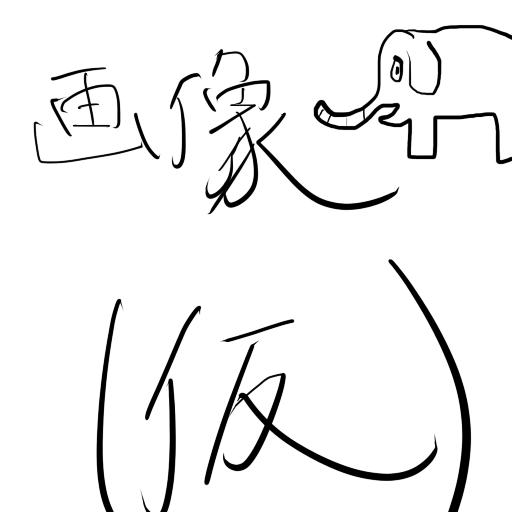
\includegraphics {kari.png}}
    \caption {初期設定画面}
    \label{honjo_ui_setup}
    \end{center}
\end{figure}

\begin{enumerate}
  \renewcommand{\labelenumi}{\textcircled{\scriptsize \theenumi}}
  \item ニックネームの入力欄\\
        ユーザがアプリ内で使用したい名前を入力します。矩形領域をタップするとキーボードが開き、入力することが可能になります。
  \item 居住地域の選択欄\\
        ユーザの住んでいる地域を選択します。矩形領域をタップするとドロップダウンリストが開き、その中から住んでいる都道府県を選択します。
  \item 完了ボタン\\
        入力が完了したら押すボタンです。入力が正しくされている場合にのみメニュー画面へ遷移することができます。
\end{enumerate}

%%%%%%%%%%%%% 子育て窓口 %%%%%%%%%%%%%%%%%%%%%%%%%%%
%% CR = Child Raising = 子育て
\subsubsection{子育て窓口}
図\ref{honjo_CR_Window}に、子育て窓口の画面を示します。
子育てにおける不安・疑問を、検索や投稿を行うことによって解決するために使用されます。

図\ref{honjo_CR_Window}に示す番号と対応させる形式で、以下にその役割を示します。

\begin{figure}[H]
    \begin{center}
    \resizebox{8cm}{!}{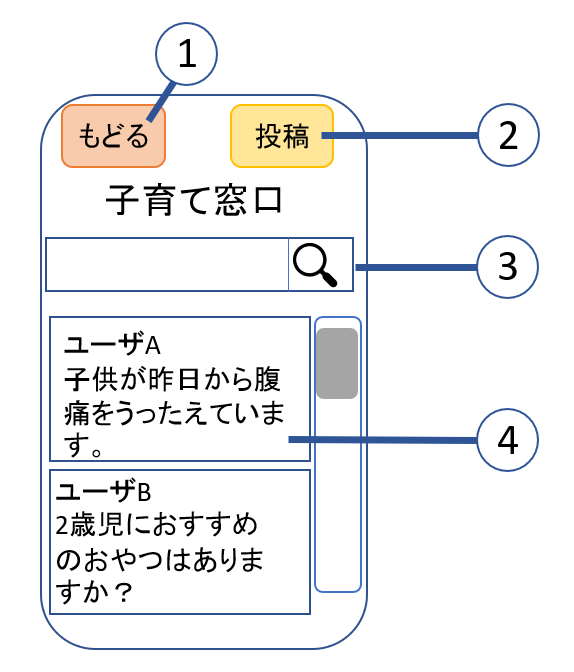
\includegraphics {honjo_CR_Window.PNG}}
    \caption {子育て窓口の画面}
    \label{honjo_CR_Window}
    \end{center}
\end{figure}

\begin{enumerate}
  \renewcommand{\labelenumi}{\textcircled{\scriptsize \theenumi}}
  \item 戻るボタン\\
        タップすると、メインメニュー画面へ遷移するボタンです。
  \item 質問投稿作成ボタン\\
        質問投稿をしたい時に押すボタンです。ペンのマークをタップすると、質問を行うための投稿画面へ遷移します。
  \item 質問の検索欄\\
        ユーザが子育て窓口内に投稿されたものを検索するために使用します。矩形領域をタップするとキーボードが開き、入力することが可能になります。
  \item 質問の一覧表示\\
        子育て窓口に投稿された質問が一覧表示されます。質問が書かれている矩形領域をタップすると質問の詳細画面へ遷移します。
\end{enumerate}

\subsubsection{質問の詳細画面}
図\ref{honjo_CR_Answer}に、質問の詳細画面を示します。
質問の詳細を閲覧、またその質問に対して回答を行うために使用されます。

図\ref{honjo_CR_Answer}に示す番号と対応させる形式で、以下にその役割を示します。

\begin{figure}[H]
    \begin{center}
    \resizebox{8cm}{!}{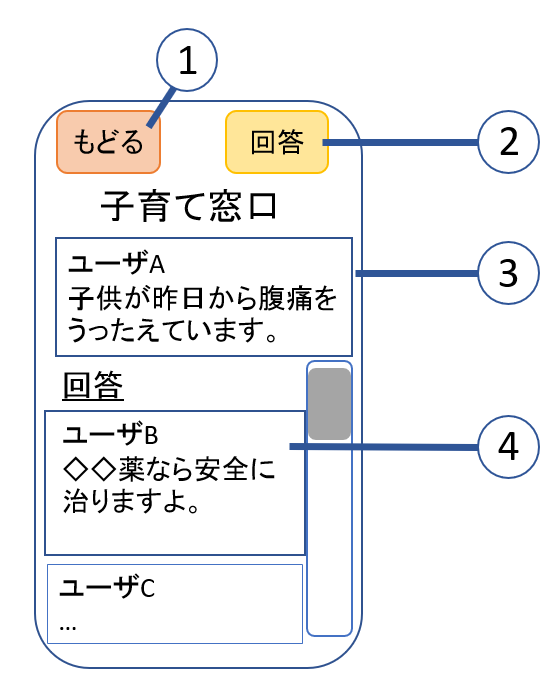
\includegraphics {honjo_CR_Answer.PNG}}
    \caption {質問の詳細画面}
    \label{honjo_CR_Answer}
    \end{center}
\end{figure}

\begin{enumerate}
  \renewcommand{\labelenumi}{\textcircled{\scriptsize \theenumi}}
  \item 戻るボタン\\
        タップすると、子育て窓口の画面へ遷移するボタンです。
  \item 回答ボタン\\
        この質問に対する回答を作成するためのボタンです。タップすると回答作成画面へ遷移します。
  \item 質問内容\\
        質問内容の全文を表示します。
  \item 回答内容\\
        回答内容の全文を表示します。複数回答がある場合は下にスクロールすることで閲覧が可能になります。
\end{enumerate}


\subsubsection{回答作成画面}
図\ref{honjo_CR_CreateAnswer}に、回答の作成画面を示します。
ある質問に対する回答を行うために使用されます。

図\ref{honjo_CR_CreateAnswer}に示す番号と対応させる形式で、以下にその役割を示します。

\begin{figure}[H]
    \begin{center}
    \resizebox{8cm}{!}{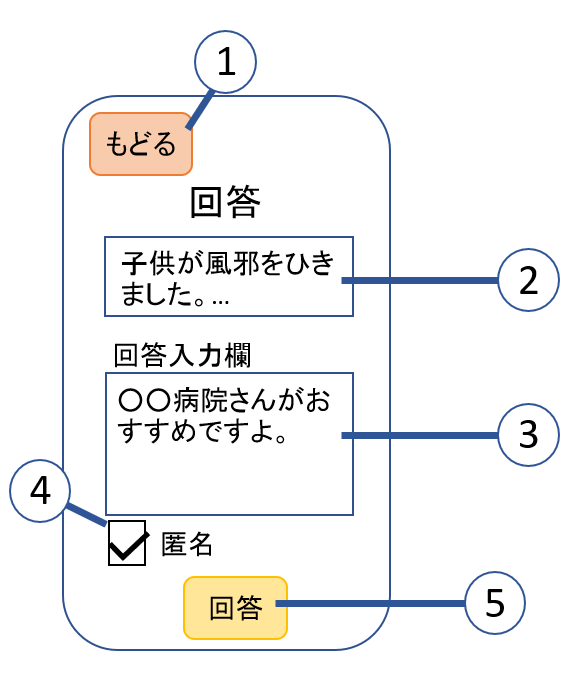
\includegraphics {honjo_CR_CreateAnswer.PNG}}
    \caption {回答作成画面}
    \label{honjo_CR_CreateAnswer}
    \end{center}
\end{figure}

\begin{enumerate}
  \renewcommand{\labelenumi}{\textcircled{\scriptsize \theenumi}}
  \item 戻るボタン\\
        タップすると、質問の詳細画面へ遷移するボタンです。
  \item 質問内容\\
        質問内容の全文を表示します。
  \item 回答内容の入力欄\\
        ユーザが回答内容を入力するための欄です。矩形領域をタップするとキーボードが開き、入力することが可能になります。
  \item 匿名チェックボックス\\
        チェックボックスをタップして、チェックが入ると、匿名で回答を投稿することが出来ます。
  \item 回答投稿ボタン\\
        回答を入力欄に書き終えて投稿をしたい時に押すボタンです。
\end{enumerate}

\subsubsection{回答投稿完了画面}
図\ref{honjo_CR_CompleteAnswer}に、質問の投稿完了画面を示します。
質問の投稿が正常に完了したことを通知するために使用されます。

図\ref{honjo_CR_CompleteAnswer}に示す番号と対応させる形式で、以下にその役割を示します。

\begin{figure}[H]
    \begin{center}
    \resizebox{8cm}{!}{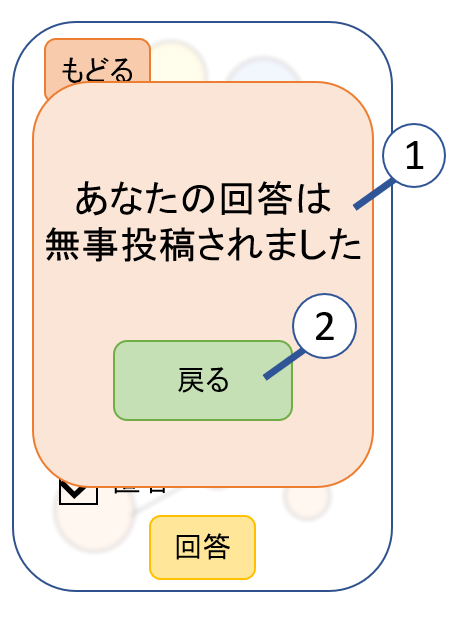
\includegraphics {honjo_CR_CompleteAnswer.PNG}}
    \caption {回答投稿画面}
    \label{honjo_CR_CompleteAnswer}
    \end{center}
\end{figure}

\begin{enumerate}
  \renewcommand{\labelenumi}{\textcircled{\scriptsize \theenumi}}
  \item ステータス\\
        ユーザの回答投稿が正常に完了したかを通知します。
  \item 戻るボタン\\
        メニュー画面へ遷移するためのボタンです。
\end{enumerate}


\subsubsection{質問投稿画面}
図\ref{honjo_CR_Contribution}に、質問の投稿画面を示します。
質問の投稿を行うために使用されます。

図\ref{honjo_CR_Contribution}に示す番号と対応させる形式で、以下にその役割を示します。

\begin{figure}[H]
    \begin{center}
    \resizebox{8cm}{!}{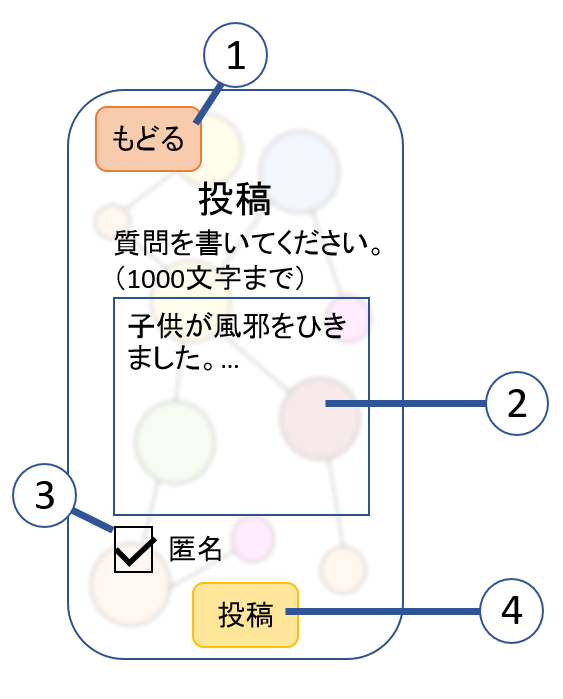
\includegraphics {honjo_CR_Contribution.PNG}}
    \caption {質問投稿画面}
    \label{honjo_CR_Contribution}
    \end{center}
\end{figure}

\begin{enumerate}
  \renewcommand{\labelenumi}{\textcircled{\scriptsize \theenumi}}
  \item 戻るボタン\\
        タップすると、子育て窓口の画面へ遷移するボタンです。
  \item 質問内容の入力欄\\
        ユーザが質問の内容を書き込むための欄です。矩形領域をタップするとキーボードが開き、入力することが可能になります。
  \item 匿名チェックボックス\\
        チェックボックスをタップして、チェックが入ると、匿名で回答を投稿することが出来ます。
  \item 投稿ボタン\\
        質問を入力欄に書き終えて投稿をしたい時に押すボタンです。
\end{enumerate}

\subsubsection{質問投稿完了画面}
図\ref{honjo_CR_CompleteContribution}に、質問の投稿完了画面を示します。
質問の投稿が正常に完了したことを通知するために使用されます。

図\ref{honjo_CR_CompleteContribution}に示す番号と対応させる形式で、以下にその役割を示します。

\begin{figure}[H]
    \begin{center}
    \resizebox{8cm}{!}{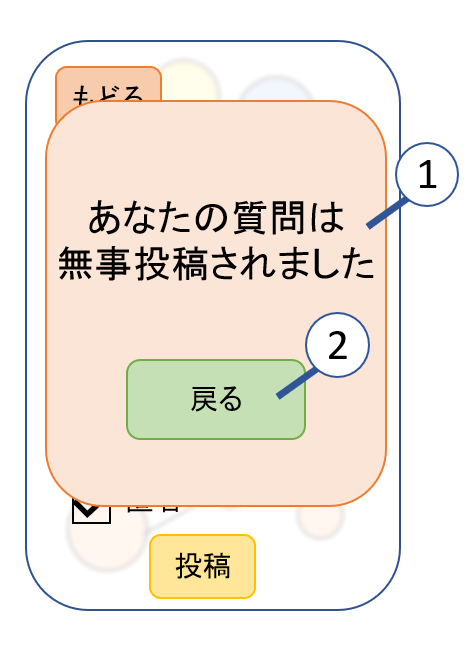
\includegraphics {honjo_CR_CompleteContribution.PNG}}
    \caption {質問投稿画面}
    \label{honjo_CR_CompleteContribution}
    \end{center}
\end{figure}

\begin{enumerate}
  \renewcommand{\labelenumi}{\textcircled{\scriptsize \theenumi}}
  \item ステータス\\
        ユーザの質問投稿が正常に完了したかを通知します。
  \item 戻るボタン\\
        メニュー画面へ遷移するためのボタンです。
\end{enumerate}

\end{document}
